\section{Experimental setup and procedure}
\label{sec:Durchführung}

\subsection{Experimental setup}
For this experiment a modified version of the thorlabs EDU-QCRY1 quantum cryptography demonstration kit \cite{thorlabs_edu-qcry1} is used.
This setup can be seen in \autoref{fig:setup_decoy}.
\\
For Alice there are two lasers of two different wavelengths.
One is green and one is red. 
Both can send laser pulses with the push of a button. 
By holding the button down, the lasers can be switched into setup mode, so that they stay on permanently for setting up the beam paths. 
In front of each laser there is a half-wave plate (HWP), whose angle can be changed, to set the basis and the content for each bit, which Alice sends to Bob. 
The two laser beams are merged with a dichroic mirror, which lets the red laser through and reflects the green laser.
\\
For Bob that kind of mirror is used to split the two laser beams again. 
Then both beams pass trough another HWP, whose angles can be altered, to set the basis, in which Bob measures the incoming Bit. 
After each HWP there is a polarizing beam splitter (PBS) which reflects one polarisation and lets the other one through. 
Two photodiodes for each differnet wavelength are placed, so that it can be determined weather the lasers were orthogonally or parallel polarized. 
For that a LED will light up, when the diode registeres an incoming pulse. 
As explained in \autoref{sec:theory}, if the basis of the incoming photons dont match the measuring basis, one photon will randomly chose one polarisation state. 
Since here the laser pulses consist of multiple photons, both photodiodes will measure the pulse. 
Therefor the randomness is here simulated by the control electronics, and only one LED will light up randomly.
The photodiodes can be set into setup mode with the press of a button, where both LED will light up in this case. 
\\
For this experiment Eve consists of one instance of Bobs setup and one instance of Alices setup. 
%\begin{figure}
%    \centering
%    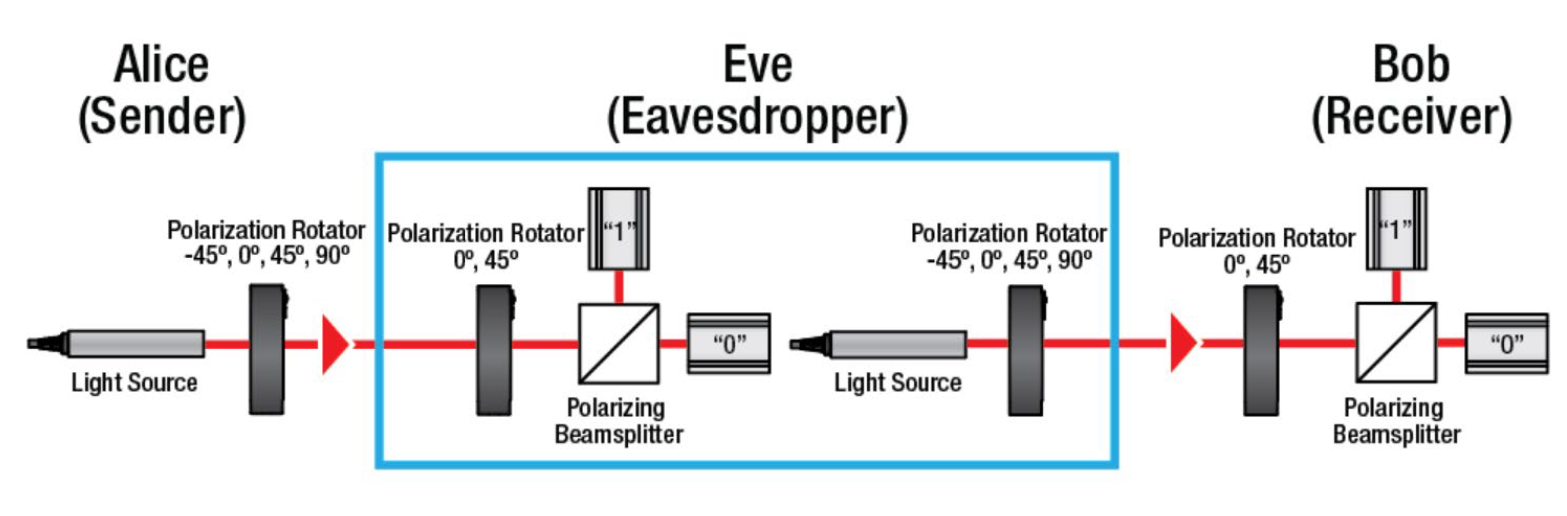
\includegraphics[width=\textwidth]{images/setup_bb84.png}
%    \caption{Experimental setup for the bb84 protocol with lasers\cite{V29}.}
%    \label{fig:setup_bb84}
%\end{figure}
\begin{figure}
    \centering
    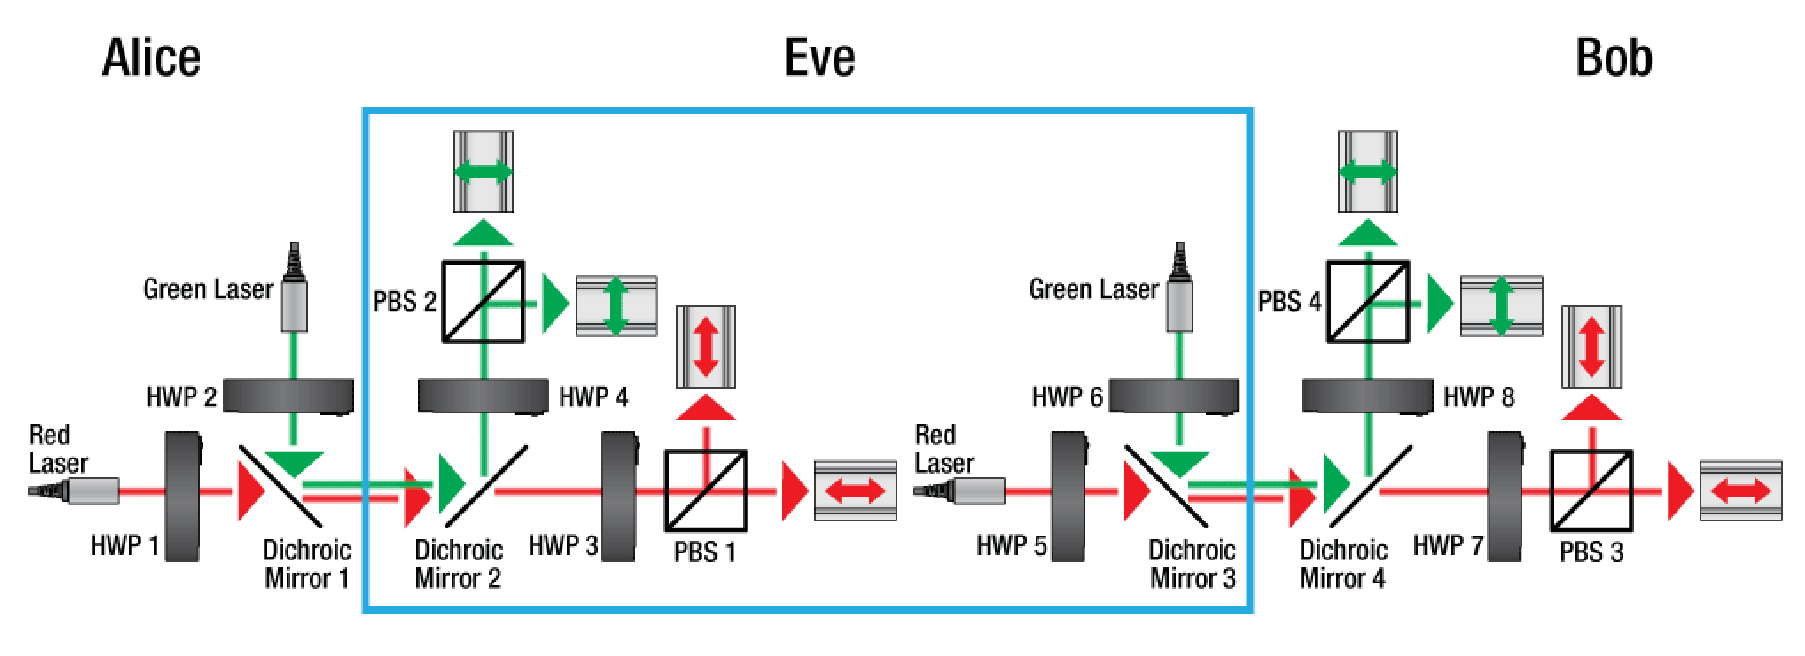
\includegraphics[width=\textwidth]{images/setup_decoy.png}
    \caption{Experimental setup for the modified bb84 protocol with lasers of two different wavelengths \cite{V29}.}
    \label{fig:setup_decoy}
\end{figure}
FloatBarrier



\subsection{Experimental procedure}

